\section{Пример использования}

Рассмотрим пример для обработки данных по численности постоянного населения Москвы и Санкт-Петербурга за период 2000-2021 годов.

Наши данные выглядят следующим образом:

\begin{figure}[H]
	\begin{center}
		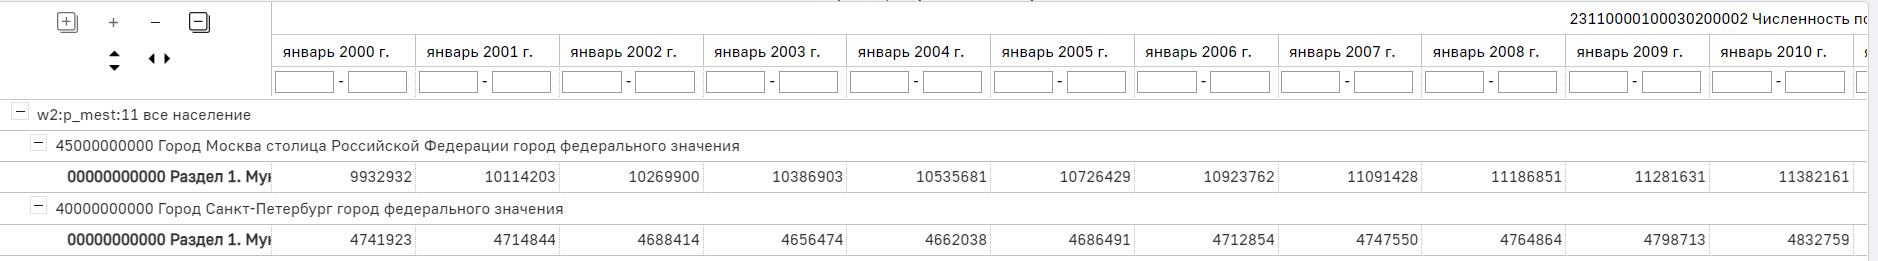
\includegraphics[scale = 0.47]{include/fig/data_rosstat}
	\end{center}
\end{figure}

Всего
\href{https://showdata.gks.ru/finder/descriptors/278928}{Росстат} выделяет нам 6 строчек, из которых нужные нам -- 4ая и 6ая.

Открываем Pycharm (Visual Studio Code) и создаем .py-файл. Перво-наперво подключаем нужные нам библиотеки и модули при помощи функции \textit{import}:

\begin{figure}[H]
	\begin{center}
		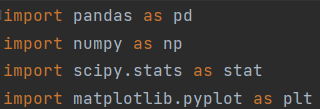
\includegraphics{include/fig/import}
	\end{center}
\end{figure}

Pandas нужен для чтения .xlsx-файла и дальнешей работы с данными; Numpy -- для работы с массивами и вычислениями основным статистик; модуль stats из библиотеки Scipy позволяет вычислять некоторые иными статистики, которых нет в Numpy; и, наконец, модуль pyplot для рисования графиков. Приписка \textit{... as ...} в каждой строчке упрощает обращение к библиотекам -- теперь нет необходимости писать её длинное название, достаточно лишь написать сокращение, которое мы сами можем выбрать.

Далее следует скачать таблицу и поместить её в одну папку с .py-файлом. Для простоты я переименовал её в "moscow\_spb.xlsx". Таким образом, воспользуемся функцией из Pandas для чтения .xlsx-файла:

\begin{figure}[H]
	\begin{center}
		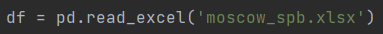
\includegraphics{include/fig/readexcel}
	\end{center}
\end{figure}

Теперь мы можем посмотреть, что внутри переменной df.

\begin{figure}[H]
	\begin{center}
		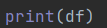
\includegraphics{include/fig/printdf}
	\end{center}
\end{figure}

И мы получим:

\begin{figure}[H]
	\begin{center}
		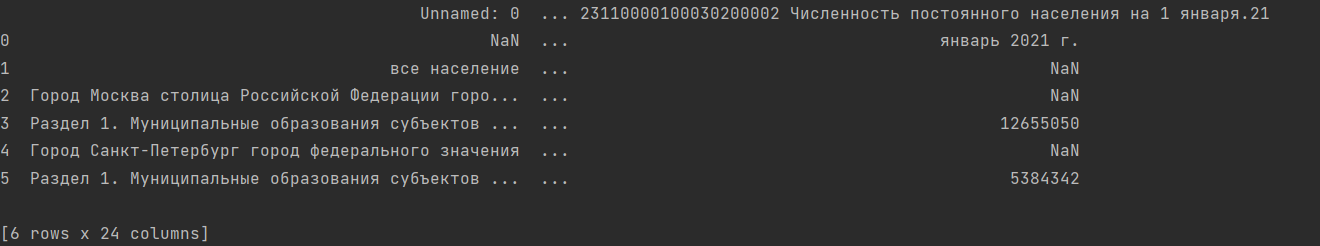
\includegraphics[scale=0.65]{include/fig/print}
	\end{center}
\end{figure}

Да, он не вывел нам всю таблицу, но можно увидеть, что сейчас в датафрейме 6 строк и 24 колонки. Изначально мы уже определили, что нам нужно 2 строчки, а период с 2000 по 2021 составляет 22 значения. Соответственно, нам необходимо "почистить" эти данные.

Со строчками мы определились выше -- 4ая и 6ая, а с колонками всё иначе. Первые две колонки содержат ненужные индексы, а их названия слишком громоздки. Программно это выглядит следующим образом:

\begin{figure}[H]
	\begin{center}
		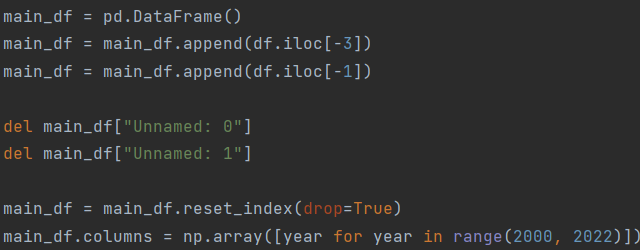
\includegraphics{include/fig/maindf}
	\end{center}
\end{figure}

Сначала мы создаем пустой датафрейм, куда мы положим нужные нам столбцы и строки. Затем мы добавляем нужную строку при помощи метода .append. То, что находится в скобках после .append -- это то, что мы добавляем в main\_df. Метод .iloc позволяет обращаться к строкам датафрейма по индексу. Этот индекс начинается с нуля, то есть, df.iloc[0] выдаст нам первую строчку, df.iloc[1] -- вторую и т.д.. Однако массивы в Python позволяют принимать отрицательные значения, что равносильно "проходу по массиву" в обратную сторону. Это значит, что df.iloc[-1] выдаст последнюю строку, а df.iloc[-3] - третью с конца. Итак, строки добавлены.

Далее мы определили, что первые две колонки содержат незначащие индексы и подписи, поэтому при помощи функции del эти колонки последовательно удаляются. Так как у них не было названия, к ним можно обратиться как "Unnamed: 0" и "Unnamed: 1" соответственно.

Если мы посмотрим на наш датафрейм сейчас, то увидим громоздкие названия столбцов и неверые индексы у строк. К названиям столбцов можно обратиться при помощи метода .columns, а присвоение чего-либо соизмеримого их просто переименует. Так показано, что мы добавляем массив (array), в котором последовательно указаны все года (все целые значения), принадлежащие полуинтервалу $\left[2000, 2022\right)$. У любого датафрейма также есть возможность сбросить по умолчанию нумерацию строк -- .reset\_index(drop=True).

"Очищенные" данные выглядят следующим образом:

\begin{figure}[H]
	\begin{center}
		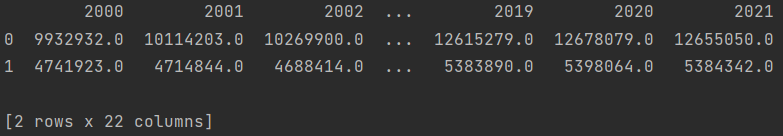
\includegraphics{include/fig/cleardf}
	\end{center}
\end{figure}

Первый город -- Москва, второй -- Санкт-Петербург. То есть, наша задача сводится к тому, чтобы пройти датафрейм построчно, описать данные и нанести их на график.

Метод .iterrows() выдает нам 2 значения -- индекс строки и саму строку. Таким образом, запустив цикл, мы можем "пройтись" по всем строкам. То есть,

\begin{figure}[H]
	\begin{center}
		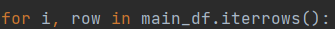
\includegraphics{include/fig/iterrows}
	\end{center}
\end{figure}

На каждой из двух итераций в переменную row будет записан массив с 22мя значениями. Для начала поделим все значения в row на 1e6, чтобы было удобнее воспринимать значения:

\begin{figure}[H]
	\begin{center}
		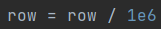
\includegraphics{include/fig/1e6}
	\end{center}
\end{figure}

Теперь можно вычислить следующие величины:

\begin{itemize}
	\item min - минимум;
	\item max - максимум;
	\item mean - среднее;
	\item median - медиана;
	\item sd (std) - стандартное отклонение;
	\item interquartile range (iqr) - интерквартильный размах;
	\item range - размах;
	\item skewness (skew) - коэффициент асимметрии;
	\item kurtosis - эксцесс.
\end{itemize}

\begin{figure}[H]
	\begin{center}
		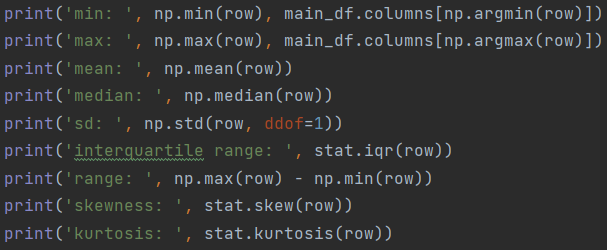
\includegraphics{include/fig/describe}
	\end{center}
\end{figure}

Наконец, построим графики.

Чтобы для каждого города отобразить отдельно 2 графика, можно воспользоваться следующим блоком кода:

\begin{figure}[H]
	\begin{center}
		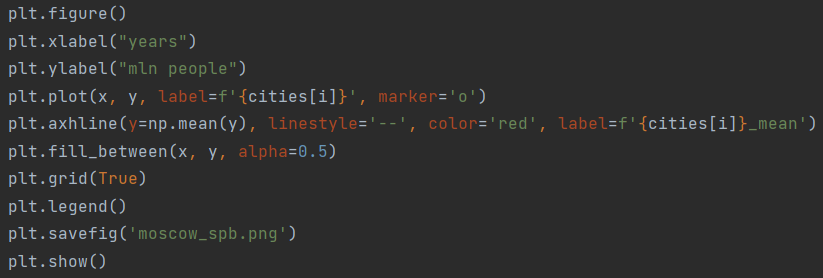
\includegraphics{include/fig/plotting}
	\end{center}
\end{figure}

Итак, 

\begin{enumerate}
	\item plt.figure() -- создает пространство для графиков;
	\item plt.xlabel("years") -- обозначает имя у оси асбцисс;
	\item plt.ylabel("mln people") -- обозначает имя у оси ординат;
	\item plt.plot(x, y, label=..., marker=...) -- наносит обычный график на пространство для графиков, подписывая его значением из \textit{label}, и маркируя каждую точку (каждое значение) фигурой из \textit{marker}. $x$ и $y$:
	
	\begin{figure}[H]
		\begin{center}
			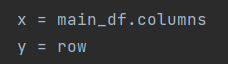
\includegraphics{include/fig/xy}
		\end{center}
	\end{figure}
	
	где $x$ -- это годы, а $y$ -- это число людей;
	
	\item plt.axhline(y=np.mean(y)) -- строит горизонтальную прямую на уровне y=np.mean(y). Для выделения этой прямой из общего графика были изменены стиль (\textit{linestyle}) и цвет (\textit{color}) линии;
	\item plt.fill\_between(x, y, alpha=0.5) -- закрашивает область под графиком с прозрачностью \textit{alpha};
	\item plt.grid() -- создает прозрачную сетку (опционально);
	\item plt.legend() -- создает легенду графика. Сюда автоматически попадают все элементы, у которых прописан параметр \textit{label};
	\item plt.savefig() -- сохраняет полученный график в файл;
	\item plt.show() -- показывает полученный график без сохранения.
\end{enumerate}

Запустив программу, в консоле мы увидим описательную статистику, а также в отдельном окне последовательно появятся два графика:

\begin{figure}[H]
	\begin{center}
		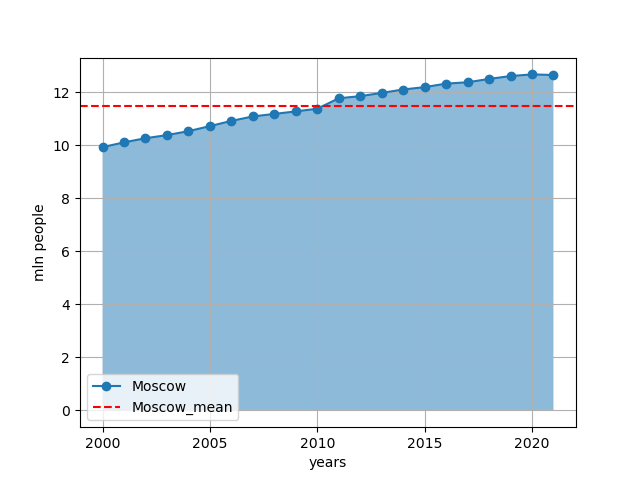
\includegraphics[scale=0.5]{include/fig/Figure_1}
		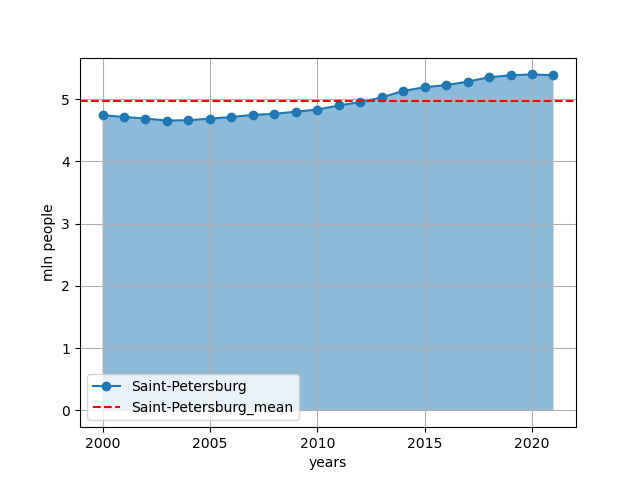
\includegraphics[scale=0.5]{include/fig/Figure_2}
	\end{center}
\end{figure}

\begin{figure}[H]
	\begin{center}
		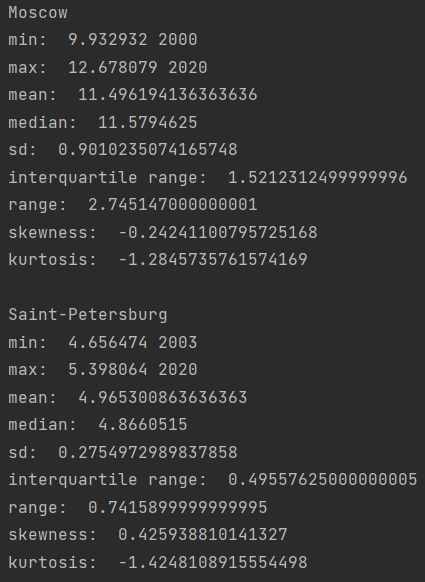
\includegraphics{include/fig/describe2}
	\end{center}
\end{figure}

Чтобы построить два графика в одном пространстве, неодходимо определить первые 3 и последние 2 строчки из блока кода выше до и после цикла "for" соответственно. Тогда получим: 

\begin{figure}[H]
	\begin{center}
		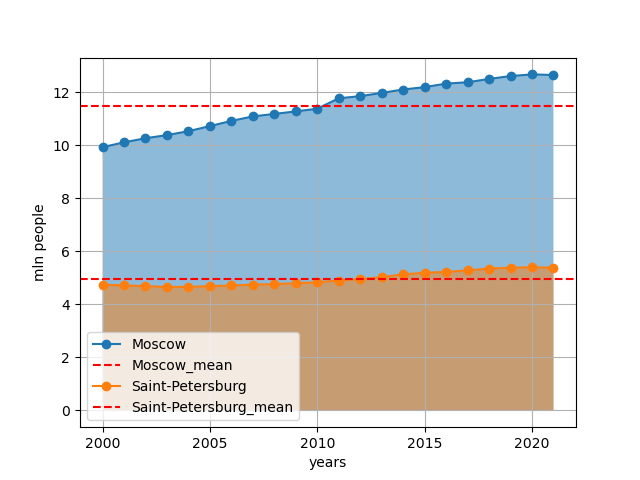
\includegraphics[scale=0.8]{include/fig/moscow_spb}
	\end{center}
\end{figure}

Полный код можно найти \href{https://github.com/Sumrak1337/statistical\_processing/blob/main/docs/example\%20of\%20usage/moscow_spb_description.py}{здесь}.

\newpage

